\documentclass[conference]{IEEEtran}

\usepackage{graphicx}
\usepackage{amsmath}
\usepackage{booktabs}   % For professional table rules
\usepackage{array}      % For column width control

\title{Weekly Report (April 07,2025 - April 13,2025)}
\author{\IEEEauthorblockN{1\textsuperscript{st}Xiaosong Yuan}
\IEEEauthorblockA{\textit{AISIG}\\
\textit{Shanghai Jiao Tong University}\\Shanghai, China\\yuanxiaosong1999@gmail.com}}

\begin{document}
\maketitle


\begin{abstract}
To bridge the knowledge gap in transitioning from undergraduate studies to Ph.D. research, this week focused on foundational learning: First, I systematically analyzed research methodologies through The Tao of Research to establish a theoretical framework for academic work. I then completed core modules of Dive into Deep Learning (Chapters 1–3), mastering linear networks, multilayer perceptrons, and optimization techniques (SGD, loss functions, softmax). Finally, I reviewed the LLM Book’s introductory chapters to reinforce prior learning. This structured approach lays the groundwork for future specialization in neural networks and machine learning.
\end{abstract}

\begin{IEEEkeywords}
research methodology, neural networks, stochastic gradient descent, loss function, scaling laws
\end {IEEEkeywords}

\section{introduction}
As my primary objective in graduate studies is to pursue and complete a Ph.D., yet recognizing my limited familiarity with advanced research methodologies, I dedicated the initial week to studying “The Tao of Research: A Path to Success in Academia” by Xiaofeng Ling. This text provided critical insights into the core responsibilities and long-term objectives of a doctoral candidate, including systematic approaches to literature review, research methodology, and identification of viable research directions. Following this theoretical foundation, I engaged with Li Mu's “Dive into Deep Learning” curriculum, completing the first three modules with particular emphasis on linear neural networks and multilayer perceptrons. This segment facilitated my comprehension of fundamental neural network architectures and associated concepts, notably stochastic gradient descent (SGD), loss function optimization, the softmax activation operator, and nonlinear activation functions. Additionally, I conducted a comprehensive review of the first two chapters of the LLM Book from prior studies to reinforce key theoretical frameworks.



\section{How to Conduct Research}
\subsection{What is a Ph.D. Student?}\label{AA}
\begin{itemize}
\item Requirements for Ph.D. Students: A Ph.D. student should complete the following cycle: “Explore new ideas → Conduct rigorous research → Publish top-tier papers → Explore new ideas → Conduct rigorous research → Publish top-tier papers…” Specifically, in the first and second years of the Ph.D., it is understandable to frequently discuss research methodologies with the advisor and refine research details under their guidance. However, by the third and fourth years, the communication with the advisor should not involve excessive details; instead, the student should independently demonstrate the ability to complete these tasks.

\item Balancing Work and Life: In the mid-to-late stages of the Ph.D., students typically spend 10–20 hours per week on teaching assistantship duties, including delivering lectures for the advisor, mentoring undergraduate or master's students, and managing research grant applications. These responsibilities hone time management and communication skills, helping them become qualified professors (independent researchers) sooner.
\end{itemize}
\subsection{How to Read Academic Papers?}\label{BB}
\begin{enumerate}
\item [a)] \textit{First Pass (Skim):} Quickly scan the entire paper to gain a general understanding of the research question, assumptions, main ideas, and proposed solutions.

\item [b)] \textit{Second Pass (Critical Thinking):} Examine the paper in detail with a critical mindset, attempting to extract new ideas and explore ways to surpass the authors' work.
\item [c)] \textit{Specific Guidelines:} Spend no more than 30\% of the time comprehending the paper’s main ideas and solutions (i.e., no more than 1–2 hours for a 10-page paper). Allocate 15 minutes to skim the abstract and introduction. If the paper is irrelevant to your research, discard it. For relevant papers, focus on understanding the algorithmic framework, experimental results, and authors' conclusions, while skimming technical details. Time Allocation: 30\% reading, 70\% critical thinking.
\item [d)]  \textit{Common Mistakes Made by Beginners:}
\begin{itemize}
\item Treating Papers Like Textbooks: Reading word-by-word as if studying a textbook is inefficient and stifles creativity. The purpose of reading academic papers is to extract new research questions and ideas—to surpass the authors’ work. Knowledge should be processed and refined by the reader’s critical thinking.
\item Going Off-Track: Spending excessive time learning technical details mentioned in the paper but unrelated to one’s research is counterproductive.
\end{itemize}
\item [e)]  \textit{Key Principle:} Engage in critical and creative thinking while reading. Prioritize need-driven learning for unfamiliar technical details—read less, think more.
\end{enumerate}



\subsection{How to Conduct Rigorous Research?}\label{CC}
\begin{itemize}
\item Define a Specific Research Question: Avoid studying random topics of interest. Instead, focus on one well-defined problem.
\item Develop Multiple Solutions: For any problem, prepare multiple candidate solutions. If one fails, proceed to the next. Pair research questions with solutions as (Problem and solution) tuples, also called research hypotheses.
\item Validate Hypotheses: A responsible researcher must rigorously test hypotheses through theoretical analysis and experimentation, providing repeated evidence to support their claims.
\item Iterate Based on Results: If both theory and experiments confirm the hypothesis, the research is temporarily complete. If either contradicts the hypothesis, switch to the next solution and restart the process.
\end{itemize}
A Useful Method for Defining Research Directions: The Chessboard Approach
\begin{figure}[htbp]
\centering
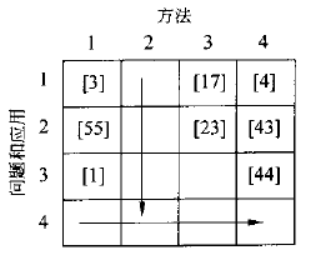
\includegraphics[width=0.3\textwidth]{./chessboard.png}
\caption{chessboard}
\label{fig:example}
\end{figure}

X-axis: Different methodologies, approaches, or techniques in the research field.

Y-axis: Research questions (or potential research problems) to be solved.

Arrange related research questions sequentially; unrelated ones can be placed arbitrarily.

Populate the chessboard with papers you have read. Empty slots represent potential research directions.

\section{In-Depth Understanding of Stochastic Gradient Descent Algorithm}
By drawing an analogy between Newton's method and stochastic gradient descent (SGD), we can gain profound insights into neural networks and the SGD algorithm.

While Newton's method may theoretically offer superior mathematical properties, stochastic gradient descent remains the predominant approach for parameter optimization in neural networks.

The fundamental principle lies in their distinct approaches: Newton's method utilizes second-order derivative information (Hessian matrix) to directly jump to the quadratic approximation's minimum point, whereas SGD iteratively follows the steepest descent direction of first-order derivatives with an appropriate learning rate to find the optimal parameters that minimize the loss function. Theoretically, Newton's method should converge faster than SGD. However, in practical applications, Newton's method is rarely employed for the following reasons:
\begin{itemize}
\item Newton's method is most effective when the loss function is convex. In practice, loss functions are typically highly complex and rarely convex (as neural networks often deal with NP-complete problems where exact solutions are unattainable). In non-convex functions, Newton's method tends to converge to saddle points rather than extremal points.

\item Modern datasets are often extremely large. Considering that the loss function is a scalar (its first derivative being a vector and its second derivative a matrix), Newton's method requires computation of both the Hessian matrix and its inverse. This leads to memory consumption scaling at O(n²) or even O(n³), which becomes computationally prohibitive for large-scale training.
\end{itemize}
Advantages of Stochastic Gradient Descent:
\begin{itemize}
\item SGD employs an iterative convergence approach, processing only small batches of data at each step, resulting in minimal memory overhead—making it ideal for massive datasets.

\item The batch-based optimization strategy avoids computing the Hessian matrix, thereby better leveraging GPU parallel computing capabilities and improving resource utilization.

\item The inherent randomness in SGD helps escape local optima.

\item The stochastic nature introduces beneficial noise during training, which in high-dimensional deep neural networks enhances model robustness and generalization capability by improving noise resistance and preventing overfitting.
\end{itemize}

\section{Deep Understanding of Cross-Entropy Loss}
\subsection{Why Use Cross-Entropy Loss Instead of MSE?}
In Softmax Regression (multinomial logistic regression), we use Cross-Entropy Loss rather than Mean Squared Error (MSE) as the loss function.
Output Mismatch
The softmax output represents a probability distribution, while MSE assumes arbitrary real-valued outputs. MSE imposes overly uniform penalties on probabilities:
For true label $y=[0,0,1]$(class 3), both predictions $\hat{y}=[0.1,0.1,0.8]$ and $\hat{y}=[0.4,0.4,0.2]$may yield similar MSE values, yet the latter completely misclassifies.
Gradient Optimization Challenges
Cross-entropy gradient is proportional to error:$\hat{y}-y$Whereas MSE gradient suffers from vanishing gradients: $(\hat{y}-y)*\hat{y}*(1-\hat{y})$.The additional $\hat{y}*(1-\hat{y})$.term approaches zero when predictions are confident $(\hat{y} \to 1)$, slowing convergence.
\subsection{Why Not Use KL-Divergence (KLD)?}
For classification tasks, cross-entropy and KLD are equivalent as both measure distribution divergence, but KLD involves redundant computations. Their relationship with entropy${H(P)}$
$$
D_{KL}(P|Q)=H(P,Q)- H(P)
$$
$$
H ( P )=-\sum_{x} P ( x ) \operatorname{l o g} P ( x )
$$
$$
D_{K L} ( P \| Q )=\sum_{x} P ( x ) \operatorname{l o g} \frac{P ( x )} {Q ( x )}
$$
$$
H ( P, Q )=H ( P )+D_{K L} ( P \| Q )=-\sum_{x} P ( x ) \operatorname{l o g} Q ( x )
$$
For one-hot encoded labels (e.g., $P=[0,1,0,0]$), $H(P)=0$ makes KLD identical to cross-entropy.

\begin{table}[!t]
\caption{Comparison Between Cross-Entropy and KL-Divergence}
\label{tab:ce_vs_kld}
\centering
\setlength{\tabcolsep}{4pt} % 减少列间距
\begin{tabular}{|p{0.22\columnwidth}|p{0.36\columnwidth}|p{0.36\columnwidth}|}
\hline
\textbf{Perspective} & \textbf{Cross-Entropy} & \textbf{KL-Divergence} \\ 
\hline 
\textbf{Math Equivalence} & 
Equivalent to KLD ($H(P)\!=\!0$) & 
Requires computing $H(P)$ \\
\hline 
\textbf{Efficiency} & 
Framework-native & 
Needs entropy computation \\
\hline 
\textbf{Gradient} & 
Identical to KLD & 
Identical \\
\hline 
\textbf{Applications} & 
Classification (one-hot) & 
Generative models \\
\hline
\end{tabular}
\end{table}



\end{document}